\section{Diskrete Bewertungsringe}

\begin{Def} 
Sei $K$ ein Körper.\\
Ein surjektiver Gruppenhomomorphismus $v: K^{\times} \to \mathbb{Z}$ heißt
\emp{diskrete Bewertung}\index{Bewertung!diskrete}, wenn für alle $x,y \in
K^{\times}$ mit $x + y \in K^{\times}$ gilt:
$$ v(x+y) \geq \min\{v(x),v(y)\}$$
Anmerkungen: Manchmal setzt man $v(0) = \infty$.\\
Da $v$ Gruppenhomomorphismus ist, gilt: $v(x \cdot y) = v(x) + v(y)$ und $v(1) = 0$.
\end{Def}

\begin{nnBsp} 
\begin{enumerate}
  \item[1.)] $K = \mathbb{Q}, \; p \in \mathbb{Z}$ Primzahl.\\
  Für $\frac{a}{b} \in \mathbb{Q} \setminus \{0\}, \; a,b \in \mathbb{Z}$
  schreibe $a = p^n \cdot a', \; b = p^m \cdot b'$ mit $p \nmid a',\; p \nmid
  b'$.\\
  Setze $v_p(\frac{a}{b}) \defeqr n - m$.
  Und es gilt: $a + b \overset{\text{\OE: } n \leq m}{=} p^n \cdot (a' + p^{m-n} b')$.\\
  $v_p$ heißt \emp{$p$-adische Bewertung}\index{Bewertung!p-adische} auf $\mathbb{Q}$. Es gilt:
  \begin{itemize}
    \item $v_p(a) \geq 0 \; \forall a \in \mathbb{Z}$. $v_3(\frac{7}{2}) = 0, \;
    v_3(\frac{9}{2})= 2$.
    \item $v_p(a+b) = \min\{v_p(a),v_p(b)\}$, falls $v_p(a) \not= v_p(b)$.
  \end{itemize}
  \item[2.)] $K = k(X) = \textrm{Quot}(k[X])$ ($k$ Körper).\\
  Für $f = \frac{f_1}{f_2}$ sei $v(f) = v(f_1) - v(f_2)$.
  \begin{enumerate}
    \item $v(f_1) = \textrm{ord}_a(f_1)$ für festes $a \in k$ (Nullstellenordnung).\\
    Es gilt $v_a(f_1 \cdot f_2) = v_a(f_1) + v_a(f_2)$\\
    $v_a(f_1 + f_2) = v_a((X-a)^{n_1} \cdot g_1 + (X-a)^{n_2} \cdot g_2)$\\
    $\overset{\text{\OE: } n_1 \leq n_2}{=} v_a((X-a)^{n_1}(g_1 + (X-a)^{n_2 - 
    n_1} \cdot g_2))$
    \item Für $f \in k[X]$ sei $v(f) = - \deg (f)$.
  \end{enumerate}
\end{enumerate}
\end{nnBsp}

\begin{Bem} 
Sei $v: K^{\times} \to \mathbb{Z}$ diskrete Bewertung.
Sei $\rho \in \mathbb{R}$ mit $0 < \rho < 1$.
Dann ist die Abbildung
$$|\;\,|_v: K \to \mathbb{R}, \; |x|_v = \begin{cases}0 &: x = 0 \\\rho^{v(x)} &: x \in K^{\times}\end{cases}$$
ein \emp{Absolutbetrag}\index{Absolutbetrag} auf $K$, d.h. eine Abbildung $K \to \mathbb{R}$ mit:
\begin{enumerate}
  \item[(i)] $|x|_v = 0 \Leftrightarrow x = 0$
  \item[(ii)] $|x \cdot y|_v = |x|_v \cdot |y|_v$
  \item[(iii)] $|x + y|_v \leq |x|_v + |y|_v$
\end{enumerate}
In unserer Situation gilt sogar:\\
$|x + y|_v \leq \max\{|x|_v,|y|_v\} \leq |x|_v + |y|_v$ $\Rightarrow$ ,,nichtarchimedischer Betrag``

Weiter ist $d(x,y) \defeqr|x - y|_v$ eine Metrik auf $K$.

\textbf{Zur Geometrie}\\
Kreis um $a$ mit Radius $r$: $K_r = \{b \in K: d(a,b) \leq r\}$.\\

\tabcolsep0mm
\begin{tabular}{lr}
\begin{minipage}{.7\textwidth}
\textbf{Jeder Kreis hat mehrere Mittelpunkte:}\\
\textbf{Beh.:} Für jedes $a' \in K_r$ ist $K_r(a') = K_r(a)$\\
\textbf{Bew.:} Sei $b \in K_r(a)$, also $d(b,a) \leq r$.\\
Dreiecksungleichung:\\
$d(b,a') \leq \max\{\underset{\leq r}{\underbrace{d(b,a)}},\underset{\leq r}{\underbrace{d(a,a')}}\} \leq r$ $\Rightarrow$ $b \in K_r(a')$
\end{minipage} &
\begin{minipage}{.3\textwidth}
\input{Algebra2Par29.pic1.pictex}
\end{minipage}
\end{tabular}

\textbf{Es gibt kein allgemeines Dreieck:}\\
Ist $d(a,b) < d(a,c)$, also $|a-b| < |c-a|$, so ist $|c-b| = |a-b+c-a| =
\max\{|a-b|,|c-a|\} = |c-a|$ $\Rightarrow$ jedes Dreieck ist gleichschenklig.
\end{Bem}

\begin{Eri}
$\mathbb{R}$ entsteht aus $\mathbb{Q}$ durch ,,Vervollständigung``:\\
$C \defeqr$ Ring der Cauchy-Folgen von $\mathbb{Q}$ (bzgl. $|\;\,|$)\\
$N \defeqr$ Ideal der Nullfolgen in $C$ (maximales Ideal)\\
$\mathbb{R} \defeqr C/N$

Analog:\\
$C_p \defeqr$ Ring der Cauchy-Folgen von $\mathbb{Q}$ (bzgl. $|\;\,|_p \defeqr |\;\,|_{v_p}$)\\
$N_p \defeqr$ Ideal der Nullfolgen in $C_p$ (maximales Ideal)\\
$\mathbb{Q}_p \defeqr C_p/N_p$ ,,\emp{Körper der $p$-adischen Zahlen}\index{p-adischen Zahlen}``
\end{Eri}

\begin{Bem}
Ist $v$ diskrete Bewertung auf $K^{\times}$, so ist $\mathcal{O}_v \defeqr \{x
\in K: v(x) \geq 0\} \cup \{0\}$ ein Ring, genauer: ein lokaler Ring mit
maximalem Ideal $\mathfrak{m}_v \defeqr \{ x \in K: v(x) > 0\} \cup \{0\}$.
\end{Bem}

\begin{Bew} 
$\mathcal{O}_v$ ist Ring, da $v(x+y) \geq \min\{v(x),v(y)\} \geq 0$ für alle
$x,y \in \mathcal{O}$.\\
$\mathfrak{m}_v$ ist Ideal: Ist $x \in \mathfrak{m}_v, \; r \in \mathcal{O}_v$, so ist $v(x \cdot r) =
v(x) + v(r) > 0$.\\
Für $x \in \mathcal{O}_v \setminus \mathfrak{m}_v = \{x \in K: v(x) = 0\}$
ist $v(\frac{1}{x})=-v(x)=0$ $\Rightarrow$ $\frac{1}{x} \in \mathcal{O}_v(\setminus
\mathfrak{m}_v)$ $\Rightarrow$ $x \in \mathcal{O}_v^{\times}$.
\end{Bew}

\begin{DefProp}
\label{2.38}
\begin{enumerate}
  \item Ein nullteilerfreier Ring $R$ heißt \emp{diskreter
  Bewertungsring}\index{Ring!diskreter Bewertungs-}, wenn es eine diskrete
  Bewertung von $K = \mathrm{Quot}(R)$ gibt mit $R = \mathcal{O}_v$.
  \item Jeder diskrete Bewertungsring ist noethersch, lokal und eindimensional.
\end{enumerate}
\end{DefProp}

\begin{Bew}
Zeige mehr: $R$ ist Hauptidealring.\\
$R$ ist lokal \checkmark, sei $\mathfrak{m}$ das maximale Ideal in $R$.\\
\textbf{Beh.1:} $\mathfrak{m}$ ist Hauptideal.\\
\textbf{Bew.1:} Sei $t \in R$ mit $v(t)=1$ $\Rightarrow$ $t \in \mathfrak{m}$. Sei $x \in \mathfrak{m}
\setminus\{0\},\; y = \frac{x}{t^{v(x)}}$ $\Rightarrow$ $v(y) = v(x) - v(t^{v(x)}) = 0$
$\Rightarrow$ $y \in R^{\times}$ $\Rightarrow$ $x = t^{v(x)} \cdot y \in (t)$.\\
\textbf{Beh.2:} Jedes Ideal $\not= 0$ in $R$ ist von der Form $\mathfrak{m}^n$ für ein $n
\geq 0$.\\
\textbf{Bew.2:} Sei $I \subseteq R$ ein Ideal, $n \defeqr \min\{v(x): x \in I
\setminus\{0\}\}$. Sei $x_0 \in I$ mit $v(x_0) = n$ $\Rightarrow$
$v(\frac{x_0}{t^n})=0$ $\Rightarrow$ $t^n = \frac{t^n}{x_0} \cdot x_0 \in I$
$\Rightarrow$ $\mathfrak{m}^n = (t^n) \subseteq I$.\\
Umgekehrt: $x_0 = t^n \cdot \frac{x_0}{t^n} \in (t^n)$.\\
Sei $x \in I$ $\Rightarrow$ $v(\frac{x}{t^n})=v(x)-n \geq 0$ $\Rightarrow$ $x = t^n \cdot \frac{x}{t^n}\in (t^n)$ $\Rightarrow$ $I \subseteq \mathfrak{m}^n$.
\end{Bew}

\begin{Satz}[Diskrete Bewertungsringe]
\label{Satz12}
Sei $R$ ein lokaler noetherscher Ring der Dimension $1$ mit maximalem Ideal
$\mathfrak{m}$ und Restklassenkörper $k = R/\mathfrak{m}$.\\
Dann sind äquivalent:
\begin{enumerate}
  \item[(i)] $R$ ist diskreter Bewertungsring
  \item[(ii)] $R$ ist (nullteilerfreier) Hauptidealring
  \item[(iii)] $R$ ist nullteilerfrei und $\mathfrak{m}$ ist ein Hauptideal
  \item[(iv)] es gibt ein $t \in R$, sodass jedes $x \in R \setminus \{0\}$ eine
  eindeutige Darstellung $x=u \cdot t^n$ hat mit $n \in \mathbb{N}, \; u \in
  R^{\times}$
  \item[(v)] $\dim_k \mathfrak{m}/\mathfrak{m}^2 = 1$
  \item[(vi)] R ist normal
\end{enumerate}
\end{Satz}

\begin{Bew}
$$
  \begin{xy}
    \xymatrix{
       (i) \ar@{=>}[rr]  &                  &  (ii) \ar@{=>}[dl] \ar@{=>}[d] \\
                         & (v) \ar@{=>}[dr] & (vi) \ar@{=>}[d] \\
       (iv) \ar@{=>}[uu] &                  & (iii) \ar@{=>}[ll]
    }
  \end{xy}
$$
\begin{description}
\item[(i) $\Rightarrow$ (ii)] \myref{Proposition}{2.38}

\item[(iv) $\Rightarrow$ (i)] $\,$\\
\underline{$R$ nullteilerfrei:}\\
Annahme: $u \cdot t^n \cdot
v \cdot t^m = 0 = u \cdot v \cdot t^{n+m}$ $\Rightarrow$ $t^{n+m} = t^{n+m} + 0 =
t^{n+m} + u \cdot v \cdot t^{n+m} = (1+u \cdot v) t^{n+m}
\overset{\text{Eind.}}{\Rightarrow} 1 + u \cdot v = 1$ $\Rightarrow$ $u \cdot v = 0
\Rightarrow$ Widerspruch zu $u \cdot v \in R^{\times}$.

\underline{Diskrete Bewertung:}\\
Für $a = u \cdot t^n \in R \setminus \{0\}$ setze $v(a) = n$.
Für $x = \frac{a}{b} \in K = \mathrm{Quot}(R), \; a,b \in R \setminus \{0\}$ setze
$v(x) = v(a) - v(b)$.

$v(x)$ wohldefiniert: Ist $x = \frac{a'}{b'}$ mit $a', b' \in R \setminus
\{0\}$, so ist $a \cdot b' =  a' \cdot b$. Aus $a = u \cdot t^n, b = v \cdot
t^m, a' = u' \cdot t^{n'}, b' = v' \cdot t^{m'}$ folgt: $u' \cdot v t^{n'+m} = u
\cdot v' \cdot t^{n + m'} \overset{\text{Eind.}}{\Rightarrow} n' + m = n + m'
\Rightarrow n'-m' = n-m$.

$v$ ist diskrete Bewertung: $v(x \cdot y) = v (u \cdot t^n \cdot v \cdot
t^m) = v(u \cdot v \cdot t^{n+m}) = n+m = v(x) + v(y)$.
$v(x + y) \overset{m < n}{=} v(t^m \cdot (v + u \cdot t^{n-m})) \geq m =
\min\{v(x),v(y)\}$.

\item[(iii) $\Rightarrow$ (iv)] Sei $\mathfrak{m} = (t)$. Sei $x \in R
  \setminus \{0\}$. Da $R$ noethersch ist, ist $\bigcap_{n \geq 0}
  \mathfrak{m}^n = (0)$ (\myref{Folgerung}{2.22}). Also gibt es ein
  (eindeutiges) $n \geq 0$ mit $x \in \mathfrak{m}^n \setminus
  \mathfrak{m}^{n+1}$ $\Rightarrow$ $\exists\, u \in R^{\times}$ mit $x = u \cdot
  t^n$.  $u$ ist eindeutig: Wäre $u \cdot t^n = v \cdot t^n$, so wäre $(u-v)
  \cdot t^n = 0$, also $t$ Nullteiler $\Rightarrow$ Widerspruch

\item[(ii) $\Rightarrow$ (v)] $\mathfrak{m}/\mathfrak{m}^2$ ist
$k$-Vektorraum: $\mathfrak{m}, \mathfrak{m}^2$ und damit
$\mathfrak{m}/\mathfrak{m}^2$ sind $R$-Moduln.
Für $a \in \mathfrak{m}$ und $x \in \mathfrak{m}/\mathfrak{m}^2$ ist $a \cdot
\bar{x} = \overline{a \cdot x} = 0$, da $a \cdot x \in \mathfrak{m}^2
\Rightarrow \bar{a} \cdot \bar{x}$ ist wohldefiniert für die Klasse $\bar{a}$
von $a$ in $R/\mathfrak{m} = k$.\\
Es ist $\mathfrak{m}^2 \not= \mathfrak{m}$, da $\dim R = 1$ (und $R$ noethersch)
$\Rightarrow \dim_k \mathfrak{m} / \mathfrak{m}^2 \geq 1$.\\
$\mathfrak{m}/\mathfrak{m}^2$ wird von $\bar{t}$ erzeugt (als $R$-Modul und
damit auch als $R/\mathfrak{m}$-Modul) $\Rightarrow \dim_k \mathfrak{m}/
\mathfrak{m}^2 \leq 1$ $\Rightarrow$ $\dim_k \mathfrak{m}/\mathfrak{m}^2 = 1$.

\item[(v) $\Rightarrow$ (iii)]
Sei $t \in \mathfrak{m}$, sodass $\bar{t} \in \mathfrak{m}/\mathfrak{m}^2$ Erzeuger ist.\\
Mit Nakayama (\myref{Folgerung}{2.21}) folgt: $t$ erzeugt $\mathfrak{m}$.

\item[(ii) $\Rightarrow$ (vi)]
Jeder (nullteilerfreie) Hauptidealring ist faktoriell\\
$\Rightarrow$ $R$ ist normal. (\myref{Bemerkung}{2.10})

\item[(vi) $\Rightarrow$ (iii)]
Sei $K = \mathrm{Quot}(R)$.\\
Sei $\bar{\mathfrak{m}} \defeqr \{x \in K: x \cdot \mathfrak{m} \subseteq
\mathfrak{m}\}$, $\mathfrak{m^{-1}} \defeqr \{x \in K: x \cdot \mathfrak{m}
\subseteq R\}$\\
Offensichtlich: $R \subseteq \bar{\mathfrak{m}} \subseteq \mathfrak{m}^{-1}$

\textbf{Beh. 1:}
\vspace{-0.7em}
\begin{enumerate}
  \item[1.)] $\bar{\mathfrak{m}} = R$
  \item[2.)] $\mathfrak{m}^{-1} \not= R$
  \item[3.)] $\mathfrak{m} \cdot \mathfrak{m}^{-1} = R$ ($\mathfrak{m} \cdot
  \mathfrak{m}^{-1}$ ist das von allen $a \cdot x, \; a \in \mathfrak{m}, \; x
  \in \mathfrak{m}^{-1}$ erzeugte Ideal in $R$)
\end{enumerate}
\vspace{-0.7em}
Dann sei $t \in \mathfrak{m} \setminus \mathfrak{m}^2$ $\Rightarrow$ $t \cdot
\mathfrak{m}^{-1} \subseteq R$ ist Ideal in $R$.
Wäre $ t \cdot \mathfrak{m}^{-1} \subseteq \mathfrak{m}$, so wäre $(t) = t \cdot
R \overset{\text{3.)}}{=} t \cdot \mathfrak{m}^{-1} \cdot \mathfrak{m} \subseteq
\mathfrak{m}^2 \Rightarrow$ Widerspruch zu $t \not\in \mathfrak{m}^2$.
Also ist $t \cdot \mathfrak{m}^{-1} = R$ und $(t) \overset{\text{3.)}}{=} t \cdot
\mathfrak{m}^{-1} \cdot \mathfrak{m} = \mathfrak{m}$.

\textbf{Bew. 3:} Aus $R \subseteq \mathfrak{m}^{-1}$ folgt $\mathfrak{m}
\subseteq \mathfrak{m} \cdot \mathfrak{m}^{-1}$. Wäre $\mathfrak{m} =
\mathfrak{m} \cdot \mathfrak{m}^{-1}$, so wäre $\mathfrak{m}^{-1} \subseteq
\bar{\mathfrak{m}} = R$ im Widerspruch zu Beh. 2.).

\textbf{Bew. 1:} $\bar{\mathfrak{m}}$ ist Unterring von $K$.\\
Zeige: $\bar{\mathfrak{m}}$ ist ganz über $R$ (dann ist $\bar{\mathfrak{m}} =
R$, da $R$ normal).\\
Es genügt zu zeigen: $\bar{\mathfrak{m}}$ ist endlich erzeugter $R$-Modul.\\
Für $t \in \mathfrak{m} \setminus \{0\}$ ist $t \cdot \bar{\mathfrak{m}}
\subseteq R$, also endlich erzeugt, da $R$ noethersch.
Als $R$-Modul sind $\bar{\mathfrak{m}}$ und $t \cdot \bar{\mathfrak{m}}$
isomorph.

\textbf{Bew. 2:} Sei $t \in \mathfrak{m} \setminus\{0\}$

\textbf{Beh. 4:} Es gibt ein $n \geq 1$ mit $\mathfrak{m}^n \subseteq (t)$.\\
Sei $n$ in Beh.4 minimal, $y \in \mathfrak{m}^{-1} \setminus (t), \; x \defeqr
\frac{y}{t} \in K$.
Dann ist $x \in \mathfrak{m}^{-1}: x \cdot \mathfrak{m} = \frac{y}{t} \cdot
\mathfrak{m} \subseteq \frac{1}{t} \cdot \mathfrak{m}^n \subseteq R$, aber $x
\not\in R$, sonst wäre $y = x \cdot t \in (t) \Rightarrow$ Widerspruch.

\textbf{Bew. 4:} $\sqrt{(t)} = \bigcap_{\mathfrak{p} \subset R, t \in
\mathfrak{p}} \mathfrak{p} = \mathfrak{m}$.\\
Seien $x_1, \dots, x_r$ Erzeuger von $\mathfrak{m}, \; \nu_i \in \mathbb{N}
\;(i=1, \dots,r)$ mit $x_i^{\nu_i} \in (t)$.\\
Für $N = 1 + \sum_{i =1}^r(\nu_i -1)$ ist dann $\mathfrak{m}^N \subseteq (t)$,
da $\mathfrak{m}^N$ erzeugt wird von den $x_1^{\nu_1} \cdot \ldots \cdot
x_r^{\nu_r}$ mit $\sum \nu_i = N$ $\Rightarrow$ $\exists\, \nu_i = 1$.
\end{description}
\end{Bew}

\tabcolsep0mm
\begin{tabular}{lr}
\begin{minipage}{.55\textwidth}
\begin{nnBsp}
$R = \left(\FakRaum{k[X,Y]}{(Y^2-X^3-X^2)}\right)_{(X,Y)}$ ist nullteilerfrei, eindimensional, lokal, noethersch aber \emph{kein} diskreter Bewertungsring.

Denn: das maximale Ideal in $R$ ist kein Hauptideal: $\mathfrak{m}=(X,Y), \; f = Y^2-X^2(X+1) \in \mathfrak{m}^2$.\\
Es gilt $\dim_k(\mathfrak{m}/\mathfrak{m}^2) = 2$, da $X,Y$ linear unabhängig in $\mathfrak{m}/\mathfrak{m}^2$.
Sei $\mathfrak{M}$ das von $X$ und $Y$ in $k[X,Y]$ erzeugte Ideal.
$\mathfrak{m}/\mathfrak{m}^2 = (\mathfrak{M}/(f))/(\mathfrak{M}^2/(f)) \cong \mathfrak{M}/\mathfrak{M}^2$\\
Geometrisch:\\
$V(f) = \{(x,y) \in k^2: \; f(x,y) = 0\} = \{ (x,y) \in k^2 : y^2 = x^2(x+1) \}$\\
Singularität in $(0,0) = (X,Y) \Rightarrow$ ``Newton-Knoten''.
\end{nnBsp}
\end{minipage} &
\begin{minipage}{.45\textwidth}
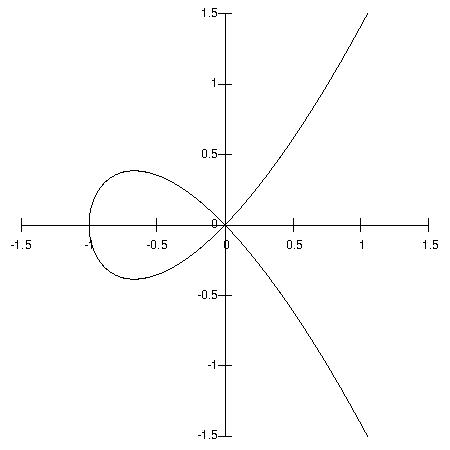
\includegraphics[width=\textwidth]{Algebra2Par29-pic2.pdf}
\end{minipage}
\end{tabular}
